\documentclass[xcolor=table, aspectratio=169, bigger, handout]{beamer}

\usepackage{shyne}

% Theme settings
\setbeamertemplate{navigation symbols}{}

\usetheme{Madrid}
\usefonttheme{structurebold}
\usefonttheme[onlymath]{serif}

\AtBeginSection[]
{ 	\begin{frame}{}

	{
	\usebeamerfont{frametitle}
	\begin{beamercolorbox}
		[wd={\textwidth}, center, sep=.2in, rounded=true, shadow=true]
		{frametitle}
	Week \thesection\\  \secname 
	\end{beamercolorbox}
	}
	
	\end{frame} 
}

\AtBeginSubsection[]
{ 	\begin{frame}{}

	{
	\usebeamerfont{frametitle}
	\begin{beamercolorbox}
		[wd={\textwidth}, center, sep=.2in, rounded=true, shadow=true]
		{frametitle}
	Section \thesection .\thesubsection\\  \subsecname 
	\end{beamercolorbox}
	}
	
	\end{frame} 
}

\title[Week 5]{Stat 201: Statistics I\\ Week 5 }
\author[M. Shyne]{}
\institute[Metro State]{
\includegraphics[width=1.75in]{../images/metro_logo}}
\date[2/10/2019]{
\\ \bigskip \bigskip 
\includegraphics[width=.4in]{../images/cc_big}}


\begin{document}
\frame{\titlepage}

%
% Week 5
%
\setcounter{section}{4}
\section{Relative Standing, Random Variables and Distributions}

%
% Section 5.1
%
\subsection{Measures of Relative Standing and Boxplots}

%%%%%%%%%%
\begin{frame}{Measures of relative standing}
\begin{block}{}
\bt{Measures of relative standing} describe the location of a given data value within a data distribution or a data set.\\
\medskip
Two measures of relative standing are discussed in this section:
\begin{itemize}
\item Z-scores
\item Percentiles
\end{itemize}
\end{block}
\end{frame}

%%%%%%%%%%
\begin{frame}{Z-scores}
\begin{block}{}
A \bt{z-score} describes the relative position of a data value within a data distribution.
\begin{itemize}
\pause
\item Another way to put it is a z-score is the number of standard deviations that a particular value is above or below the mean.
\pause
\item Z-scores are standardized and unit-less, so they can be used to compare values from different populations.
\pause
\item A positive z-score means the value is greater than the mean and a negative z-score means that it is below the mean. 
\pause
\item Z-scores can be calculated for samples or populations, if the population mean and standard deviation are known.
\end{itemize}
\end{block}
\end{frame}

%%%%%%%%%%
\begin{frame}{Z-scores, calculations}
\begin{block}{To calculate}
\begin{itemize}
\item For a sample $X$ with sample mean $\bar x$ and standard deviation $s$, the z-score for a value $x$ is\\ \smallskip
\eq{z = \frac{x - \bar x}{s}}
\smallskip
\pause
\item For a population with population mean $\mu$ and standard deviation $\sigma$, the z-score for value $x$ is\\ \smallskip
\eq{z = \frac{x - \mu}{\sigma}}
\end{itemize} 
\end{block}
\end{frame}

%%%%%%%%%%
\begin{frame}{Z-scores, example}
\begin{exampleblock}{Example}
Recall the example of a sample of student ages. The sample has ages $X = \set{22, 32, 46, 50, 33, 38, 20, 24}$, with a mean of $\bar x = 33.125$ and standard deviation of $s=11.05$.
\begin{itemize}
\pause
\item Suppose a new student joins the class. His age is 61. He has an age $z$-score of\\ \smallskip
\eq{z = \frac{x - \bar x}{s} = \frac {61-33.125}{11.05} = \frac {27.875}{11.05} = 2.52}
\medskip
\pause
His age two and a half standard deviations above the class mean.
\smallskip
\pause
\item Another student joins the class. Her age is 27. She has an age $z$-score of\\
\smallskip
\eq{z = \frac{x - \bar x}{s} = \frac {27-33.125}{11.05} = \frac {-6.125}{11.05} = -0.554}
\medskip
\pause
Her age is about a half standard deviation below the class mean.
\end{itemize}

\end{exampleblock}
\end{frame}

%%%%%%%%%%
\begin{frame}{Values from z-scores}
\begin{block}{}
Sometimes, it is useful to find a value within a data distribution that corresponds to a given z-score. That is, find an $x$ given a $z$. 
\medskip
\begin{itemize}
\pause\item Start with the z-score equation, \\
\smallskip
\eq{z = \frac{x - \bar x}{s} \txtor z = \frac{x - \mu}{\sigma}}
\pause\item After some algebra,\\
\smallskip
\eq{x = \bar x + z s \txtor x = \mu + z \sigma}
\end{itemize}
\end{block}

\pause
\begin{exampleblock}{Example}
What age is 2 standard deviations above the mean for this data? That is, what age corresponds to $z=2$?\\
\smallskip
\pause
\eq{x = \bar x + z s = 33.125 + 2 \times 11.05 =  55.225 \text{ years}}
\end{exampleblock}
\end{frame}

%%%%%%%%%%
\begin{frame}{Unusual/significant values}

{\centering
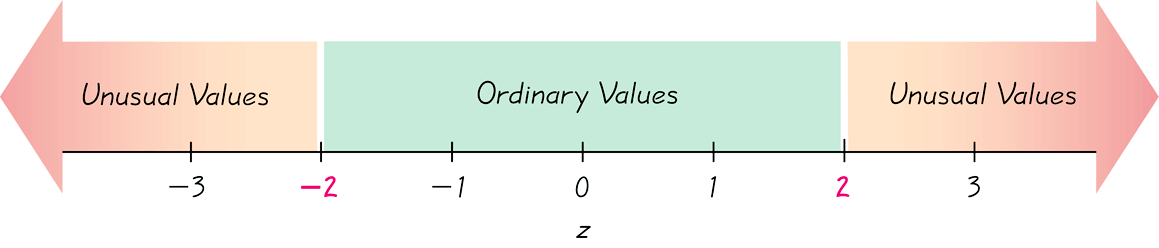
\includegraphics[width=4.5in]{../images/ch03_unusual} \par
}

\begin{block}{}
A value is called \bt{unusual or significant} if it has a z-score $z$ such that $z< -2$ or $z > 2$. A value is \bt{ordinary} if $z$ is between $-2$ and $2$.
\end{block}

\pause
\begin{exampleblock}{Example}
Consider the new students to the class:
\begin{itemize}
\item The 61 year old ($z=2.52$) has an unusual age for the class. 
\item The 27 year old ($z=-0.554$) has an ordinary age for the class.
\end{itemize}
\end{exampleblock}
\end{frame}

%%%%%%%%%%
\begin{frame}{Percentiles}
\begin{block}{}
\bt{Percentiles} measure relative position within a data set as order rank expressed as a percent. In other words, the value at the $p$th percentile (written as $P_p$) in a data set is greater than $p$\% of the data.
\end{block}

\pause

\begin{exampleblock}{Example}
Percentiles are often used in reporting scores on standardized tests.\\
\medskip
Suppose a student scores in the 83rd percentile on the ACT. That means she scored better than 83\% of the students who took the ACT.
\end{exampleblock}
\end{frame}

%%%%%%%%%%
\begin{frame}{Calculate percentiles}
\begin{block}{To calculate}
\begin{itemize}
\item To find the percentile of a value $x$ in a data set,\\
\smallskip
\eq{\%\text{ile} = \frac{\text{number of values} < x}{n} \times 100\%}
\medskip
If percentile is not a whole number, round up.
\medskip
\pause\item To find the value of $P_p$ (the $p$th percentile), calculate the rank,\\
\smallskip
\eq{r = \frac p {100} \times n}
\medskip
If $r$ is a whole number, $P_p$ is the mean of the $r$th and $(r+1)$th values. If not, round up. Then, $P_p$ is the $r$th value in an ordered list.
\end{itemize}
\end{block}
\end{frame}

%%%%%%%%%%
\begin{frame}{Percentile, example}
\begin{exampleblock}{Example}
The age data, in order is, \\
\smallskip
\eq{20 \quad 22 \quad 24 \quad 32 \quad 33 \quad 38 \quad 46 \quad 50}

\begin{itemize}
\pause
\item The percentile of the value 38 is\\
\smallskip
\eq{\frac{\text{number of values} < x}{n} \times 100\% = \frac{5}{8} \times 100\% = 62.5 \,\% \implies P_{63}} 
\medskip
\pause\item To find the 30th percentile, $P_{30}$, calculate rank\\
\smallskip
\eq{r= \frac {p}{100} \times n = \frac {30}{100} \times 8 = 2.4 }
\medskip
Round up $r$ to $3$. $P_{30}$ is the 3rd value, $24$.
\end{itemize}
\end{exampleblock}
\end{frame}

%%%%%%%%%%
\begin{frame}{Quartiles}
\begin{block}{}
The \bt{quartiles} are values that divide the data set into 4 parts, or quarters.\\
\smallskip
\eq{Q_1 = P_{25} \qquad Q_2 = P_{50} \qquad Q_3 = P_{75}}
\begin{itemize}
\pause
\item Note: The median is equivalent to $Q_2$ and $P_{50}$.
\end{itemize}
\end{block}
\end{frame}

%%%%%%%%%%
\begin{frame}{5 number summary}
\begin{block}{}
The \bt{5 number summary} summarizes the distribution of a data set.\\
\medskip
The 5 numbers are:
\begin{itemize}
\item Minimum
\item $Q_1$
\item Median (or $Q_2$)
\item $Q_3$
\item Maximum
\end{itemize}
\end{block}
\end{frame}

%%%%%%%%%%
\begin{frame}{5 number summary, example}
\begin{exampleblock}{Example}
The age data, in order is, \\ \smallskip
\eq{20 \quad 22 \quad 24 \quad 32 \quad 33 \quad 38 \quad 46 \quad 50}
\medskip
The 5 number summary is\\ \smallskip
\eq{\underbrace{20}_{\min} \quad \underbrace{23}_{Q_1} \quad \underbrace{32.5}_{\f{med}} \quad \underbrace{42}_{Q_3} \quad \underbrace{50}_{\max}}
\end{exampleblock}
\end{frame}

%%%%%%%%%%
\begin{frame}{Boxplots}
\begin{block}{}
A \bt{boxplot} is a graph depicting the 5 number summary.
\begin{itemize}
\item $\set{20,  23, 32.5, 42, 50}$
\end{itemize}
\end{block}
{\centering
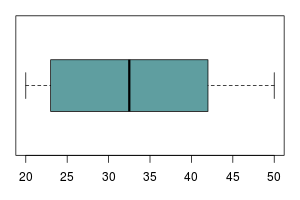
\includegraphics[width=3.5in]{../images/wk05_boxplot}\par
}
\end{frame}


%%%%%%%%%%
\begin{frame}<handout:0>{Group work}
\begin{block}{}
\large
\begin{itemize}
\item Complete question 1.
\end{itemize}
\end{block}
\end{frame}



%
% Section 5.2
%
\subsection{Probability Distributions}

%%%%%%%%%%
\begin{frame}{Random variables}
\begin{block}{}
A \bt{random variable} is a variable that has a numeric value determined by chance from a range of possible values.

\begin{itemize}
\pause\item An outcome of a trial
\pause\item Usually designated with a capital letter ($X, \, Y,$ etc.)
\pause\item Lowercase letters refer to specific values of the random variable
\pause\item Thus, $P(X=x)$ means the probability that the random variable $X$ takes the specific value $x$.
\end{itemize}
\end{block}
\end{frame}


%%%%%%%%%%
\begin{frame}{Random variables, examples}
\begin{exampleblock}{Example}
\begin{itemize}
\item $X$ = the number of heads from three coin flips
\item $Y$ = the sum of two dice
\item $Z$ = the midterm score of a randomly selected student
\begin{itemize}
\item A students grade (A, A-, B+, etc.) can not be used as a random variable because it is not numeric,
\item ... Unless the grade is coded as a number (i.e. A = 4.0, A- = 3.7, etc.)
\end{itemize}
\end{itemize}
\end{exampleblock}
\end{frame}

%%%%%%%%%%
\begin{frame}{Types of random variables}
\begin{block}{}
Recall, numeric variables can be classified as \bt{discrete} or \bt{continuous}. Random variables also can be either discrete or continuous.
\end{block}

\pause
\begin{exampleblock}{Example}
Discrete random variables:
\begin{itemize}
\item Number of heads on three coin flips
\item Number of defective insulin test strips in a box of 50
\item Number of customers to enter a store in the next 10 minutes
\end{itemize}
\pause
Continuous random variables:
\begin{itemize}
\item Height or weight of a test subject
\item Survival time of a cancer patient
\item Price of a company's stock at a particular moment
\end{itemize}
\end{exampleblock}
\end{frame}

%%%%%%%%%%
\begin{frame}{Probability distributions}
\begin{block}{}
The collection of probabilities of all the possible values of a random variable is known as the \bt{probability distribution} of the random variable.

\begin{itemize}
\pause\item Each probability is between 0 and 1
\pause\item The probabilities must add up to 1
\pause\item Often displayed in tables (if practical)
\end{itemize}
\end{block}
\end{frame}

%%%%%%%%%%
\begin{frame}{Probability distributions, example}
\begin{exampleblock}{Example}
A restaurant wants to track its taco sales. It records how many tacos customers order with each visit. The results are in the table,\\
\medskip
{\centering \tabspacemed
\begin{tabular}{r | c cccc}
Number of tacos & 0 & 1 & 2 & 3 & 4\\
\hline
Probability &  0.35 & 0.2 & 0.3 & 0.1 & 0.05
\end{tabular}\par
}
\medskip
Is this a probability distribution?
\begin{itemize}
\pause\item These are probabilities of every possible outcome of a trial (customer making an order).
\pause\item The probabilities add to 1.
\pause\item It is a probability distribution.
\end{itemize}
\end{exampleblock}
\end{frame}

%%%%%%%%%%
\begin{frame}{Probability distributions, example}
\begin{exampleblock}{Example}
The restaurant introduces a new "Super Taco" (beef, chicken and shrimp). It wonders if larger groups are more likely to order the new item. The results are in the table,\\
\medskip
{\centering \tabspacemed
\begin{tabular}{r | cccc}
Number in group & 1 & 2 & 3 & 4 or more \\
\hline
Probability of ordering & 0.05 & 0.03 & 0.04 & 0.15
\end{tabular}\par
}
\medskip
Is this a probability distribution?
\begin{itemize}
\pause\item The probabilities are for a different event (ordering a Super Taco) than the values (number in group). 
\pause\item The probabilities do not add to 1.
\pause\item It is not a probability distribution.
\end{itemize}
\end{exampleblock}
\end{frame}

%%%%%%%%%%
\begin{frame}{Event probabilities}
\begin{block}{}
To calculate the probability of an event given a probability distribution, simply add the probabilities of the outcomes which comprise the event.
\end{block}
\pause
\begin{exampleblock}{Example}
{\centering \tabspacemed
\begin{tabular}{r | c cccc}
Number of tacos & 0 & 1 & 2 & 3 & 4\\
\hline
Probability &  0.35 & 0.2 & 0.3 & 0.1 & 0.05
\end{tabular}\par
}
\bigskip
What is the probability of a customer ordering less than two tacos?\\ \smallskip
\pause
\eq{P(X<2) = P(X = 0 \text{ or } X = 1) = P(0) + P(1) = 0.35 + 0.2 = 0.55}
\end{exampleblock}
\end{frame}

%%%%%%%%%%
\begin{frame}{Weighted means}
\begin{block}{}
A \bt{weighted mean} is the mean of values that are not considered equally, or do not have equal importance.
\begin{itemize}
\item Each value has an associated weight, which is its relative importance.
\item To calculate, let $x_i$ be a value and $w_i$ its weight. \\ \smallskip
\eq{\mu_w = \frac {\sum w_i \times x_i}{\sum w_i}}
\end{itemize}
\end{block}
\pause
\begin{exampleblock}{Example}
Fiona buys 4 lbs. of hamburger at \$4.89 / lb. and 2 lbs. of steak at \$11.99 / lb. What is the average price per pound she is paying?\\ \smallskip 
\pause
\eq{ \$/lb. = \frac {4 \times 4.89 + 2 \times 11.99}{6} = \frac {43.54}{6} = 7.26 }
\end{exampleblock}
\end{frame}

%%%%%%%%%%
\begin{frame}{Mean of probability distributions}
\begin{block}{}
The mean of a probability distribution is a weighted mean of the possible values, with the probability of each as its weight. 

\begin{itemize}
\pause\item Since the sum of probabilities of a distribution is always 1, the divisor of the weighted mean is 1 which we can ignore.
\pause\item Thus, the mean is\\ \smallskip
\eq{\mu = \sum x_i \cdot P(x_i) }
\end{itemize}
\medskip
\pause
The mean of a probability distribution is also known as the \bt{expected value} of the random variable (or sometimes as just the mean of the random variable).
\begin{itemize}
\item Denoted with an ``E", as in \\ \smallskip
\eq{\E(X) = \mu }
\end{itemize}
\smallskip
\end{block}
\end{frame}

%%%%%%%%%%
\begin{frame}{Mean, example}
\begin{exampleblock}{Example}
{\centering \tabspacemed
\begin{tabular}{r | c cccc}
Number of tacos & 0 & 1 & 2 & 3 & 4\\
\hline
Probability &  0.35 & 0.2 & 0.3 & 0.1 & 0.05
\end{tabular}\par
}
\bigskip

What is the mean number of tacos ordered at the restaurant? That is, how many tacos should the restaurant expect each customer to order?\\
\medskip
\pause
{\centering 
\begin{tabular}{r l}
$\E(X) = \mu =$ & $\sum x_i \cdot P(x_i)$\\
$=$ & $(0 \cdot 0.35) + (1 \cdot 0.2) + (2 \cdot 0.3) + (3 \cdot 0.1)+ (4 \cdot 0.05)$\\
$=$ & 0 + 0.2 + 0.6 + 0.3 + 0.2\\
$=$ & 1.3
\end{tabular}\par
\renewcommand{\arraystretch}{1.5}}

\end{exampleblock}
\end{frame}

%%%%%%%%%%
\begin{frame}{Standard deviation of probability distributions}
\begin{block}{}
Similarly, variance of a probability distribution is the weighted mean of difference from the mean squared and standard deviation is the square root of variance.\\
\medskip
Thus, \\ \smallskip
\eq{\sigma^2 = \sum (x_i - \bar x )^2 \cdot P(x_i)}
\eq{\sigma = \sqrt{\sigma^2}}
\end{block}
\end{frame}

%%%%%%%%%%
\begin{frame}{Standard deviation, example}
\begin{exampleblock}{Example}
What is the standard deviation of number of tacos ordered at the restaurant?\\
\medskip
\pause
{\centering
\begin{tabular}{r l}
$\sigma^2 =$ & $\sum (x_i - \mu )^2 \cdot P(x_i)$\\
$=$ & $(0-1.3)^2 \cdot 0.35 + \cdots + (4-1.3)^2 \cdot 0.05$\\
$=$ & $0.5915 + \cdots + 0.3645$\\
$=$ & $1.41$\\
\pause$\sigma = \sqrt{\sigma^2} = $ & $1.19$
\end{tabular}\par
\renewcommand{\arraystretch}{1.5}}
\end{exampleblock}
\end{frame}


%%%%%%%%%%
\begin{frame}{Unusual/significant events}
\begin{block}{}
If the probability of a random variable being equal to an event or takes a value more extreme than than the event is less than some threshold, usually 0.05, then the event is an \bt{unusual or significant event}.\\
\medskip
\pause
That is, if $x$ is an extreme value if\\ \medskip
\eq{P(X \le x) < 0.05 \txtor P(X \ge x) < 0.05}
\medskip
\end{block}
\end{frame}

%%%%%%%%%%
\begin{frame}{Unusual/significant events, example}
\begin{exampleblock}{Example}
Tom and Barbara collect eggs from their chickens everyday. The number of eggs they collect follows the following distribution,\\
\smallskip
{\centering
\begin{tabular}{c|cccccccccc}
Eggs ($x$) & 0 & 1 & 2 & 3 & 4 & 5 & 6 & 7 & 8 & 9 \\
\hline
$P(x)$ & 0.01 & 0.03 & 0.1 & 0.2 & 0.3 & 0.2 & 0.1 & 0.04 & 0.02 & 0
\end{tabular}\par
}
\medskip
Is collecting 1 egg significantly low? Is collecting 7 eggs significantly high?
\begin{itemize}
\pause\item $P(X\le 1) = P(0) + P(1) = 0.04  < 0.05$\\
\bt{Collecting 1 egg is significantly low.}
\pause\item $P(X \ge 7) = P(7) + P(8) + P(9) = 0.06 \not < 0.025$\\
\bt{Collecting 7 eggs is not significantly high.}
\end{itemize}
\end{exampleblock}
\end{frame}

%%%%%%%%%%
\begin{frame}{Rare event rule}
\begin{block}{}
The \bt{rare event rule} says that if observed results are unusual, given an assumed probability distribution, then perhaps the assumption is wrong.
\end{block}
\pause
\begin{exampleblock}{Example}
Recall the example of flipping a coin 1000 times. Under the assumption the coin is fair ($P(H) = P(T) = 1/2$), the expected number of heads is 500.
\begin{itemize}
\pause\item Getting 523 heads is not unusual ($P(X \ge 523) = 0.077$). There is no reason to think the coin is not fair.
\pause\item Getting 46 heads is unusual ($P(X \le 46) = 6.23 \times 10^{-222}$). We would be justified in questioning the assumption that the coin is fair.
\end{itemize}
\end{exampleblock}
\end{frame}



%%%%%%%%%%
\begin{frame}<handout:0>{Group work}
\begin{block}{}
\large
\begin{itemize}
\item Complete question 2.
\end{itemize}
\end{block}
\end{frame}






\end{document}